\documentclass[handout]{beamer}


\usetheme{default}
\usepackage{subfigure}
\usepackage{amsmath}
\usepackage{Sweave}
\usepackage{graphicx}
\usepackage{color}
\usepackage{amsfonts}
\usepackage{amssymb}
\usepackage{multicol}
\usepackage[all]{xy}
\usepackage{bm}


\author{Patrick Lam}
\title{Convergence Diagnostics}
\date{}
%\date{November 10, 2008}

\begin{document}

\newcommand{\red}{\textcolor{red}}
\newcommand{\blue}{\textcolor{blue}}
\newcommand{\purple}{\textcolor{purple}}

\frame{\titlepage}

\begin{frame}
\frametitle{Outline}
\tableofcontents
\end{frame}


\section{Convergence}

\begin{frame}
\frametitle{Outline}
\tableofcontents[currentsection]
\end{frame}


\begin{frame}[fragile]
\frametitle{Running Example}
\pause
As a running example, we will use the bivariate normal Metropolis
sampler from class.
\medskip
\pause
\tiny
\begin{Schunk}
\begin{Sinput}
> NormalMHExample <- function(n.sim, n.burnin) {
+     library(mvtnorm)
+     mu.vector <- c(3, 1)
+     variance.matrix <- cbind(c(1, -0.5), c(-0.5, 2))
+     theta.mh <- matrix(NA, nrow = n.sim, ncol = 2)
+     theta.current <- rnorm(n = 2, mean = 0, sd = 4)
+     theta.update <- function(index, theta.current, ...) {
+         theta.star <- rnorm(n = 1, mean = theta.current[index], sd = 2)
+         if (index == 1) 
+             theta.temp <- c(theta.star, theta.current[2])
+         else theta.temp <- c(theta.current[1], theta.star)
+         r <- dmvnorm(theta.temp, mu.vector, variance.matrix)/dmvnorm(theta.current, 
+             mu.vector, variance.matrix)
+         r <- min(r, 1, na.rm = T)
+         if (runif(1) < r) 
+             theta.star
+         else theta.current[index]
+     }
+     for (i in 1:n.sim) {
+         theta.current[1] <- theta.mh[i, 1] <- theta.update(1, theta.current, 
+             mu.vector, variance.matrix)
+         theta.current[2] <- theta.mh[i, 2] <- theta.update(2, theta.current, 
+             mu.vector, variance.matrix)
+     }
+     theta.mh <- theta.mh[(n.burnin + 1):n.sim, ]
+ }
> mh.draws <- NormalMHExample(n.sim = 5000, n.burnin = 0)
\end{Sinput}
\end{Schunk}
\normalsize
\end{frame}


\begin{frame}
\frametitle{Convergence}
\pause
From our theory of Markov chains, we expect our chains to eventually
converge to the stationary distribution, which is also our target
distribution. \\
\pause
\bigskip
However, there is no guarantee that our chain has converged after $M$ draws.\\
\pause
\bigskip
How do we know whether our chain has actually converged? \\
\pause
\bigskip
We can never be sure, but there are several tests we can do, both
visual and statistical, to see if the chain appears to be converged.
\end{frame}

\begin{frame}[fragile]
\frametitle{Convergence Diagnostics in R}
All the diagnostics we will use are in the {\tt coda} package in R.
\medskip
\pause
\tiny
\begin{Schunk}
\begin{Sinput}
> library(coda)
\end{Sinput}
\end{Schunk}
\normalsize
\bigskip
\pause
Before we use the diagnostics, we should turn our chains into {\tt
mcmc} objects.
\medskip
\pause
\tiny
\begin{Schunk}
\begin{Sinput}
> mh.draws <- mcmc(mh.draws)
\end{Sinput}
\end{Schunk}
\bigskip
\normalsize
\pause
We can tell the {\tt mcmc()} function to burn-in or drop draws with
the {\tt start} and {\tt end} arguments. \\
\bigskip
\pause
{\tt mcmc()} also has a {\tt thin} argument, which only tells it the
thinning interval that was used (it does not actually thin for us).
\end{frame}

\begin{frame}[fragile]
\frametitle{Posterior Summary}
\pause
We can do {\tt summary()} of an {\tt mcmc} object to get summary
statistics for the posterior.
\medskip
\pause
\tiny
\begin{Schunk}
\begin{Sinput}
> summary(mh.draws)
\end{Sinput}
\begin{Soutput}
Iterations = 1:5000
Thinning interval = 1 
Number of chains = 1 
Sample size per chain = 5000 

1. Empirical mean and standard deviation for each variable,
   plus standard error of the mean:

       Mean    SD Naive SE Time-series SE
[1,] 3.0282 1.027  0.01453        0.03859
[2,] 0.9997 1.424  0.02014        0.04109

2. Quantiles for each variable:

       2.5%     25%    50%   75% 97.5%
var1  0.864 2.37214 3.0489 3.733 5.016
var2 -1.622 0.03447 0.9984 1.927 3.777
\end{Soutput}
\end{Schunk}
\bigskip
\pause
\normalsize
The results give the posterior means, posterior standard deviations,
and posterior quantiles for each variable. 
\end{frame}

\begin{frame}
The ``na\"{\i}ve'' standard error is the \textbf{standard error of the mean},
which captures \textit{simulation error} of the mean rather than posterior
uncertainty.  
\pause
\begin{eqnarray*}
\mathrm{naive \; SE} = \frac{\mathrm{posterior \; SD}}{\sqrt{n}}
\end{eqnarray*}
\pause
The time-series standard error adjusts the ``na\"{\i}ve'' standard
error for autocorrelation.
\end{frame}


\section{Visual Inspection}

\begin{frame}
\frametitle{Outline}
\tableofcontents[currentsection]
\end{frame}

\begin{frame}
\frametitle{Mixing}
\pause
One way to see if our chain has converged is to see how well our chain
is \textbf{mixing}, or moving around the parameter space.\\
\pause
\bigskip
If our chain is taking a long time to move around the parameter space,
then it will take longer to converge.  \\
\pause
\bigskip
We can see how well our chain is mixing through visual inspection. \\
\pause
\bigskip
We need to do the inspections for every parameter.
\end{frame}

\begin{frame}
\frametitle{Traceplots}
\pause
A \textbf{traceplot} is a plot of the iteration number against the
value of the draw of the parameter at each iteration.\\
\pause
\bigskip
We can see whether our chain gets stuck in certain areas of the
parameter space, which indicates bad mixing.

\pause

\begin{figure}[!htp]
\begin{center}
\subfigure{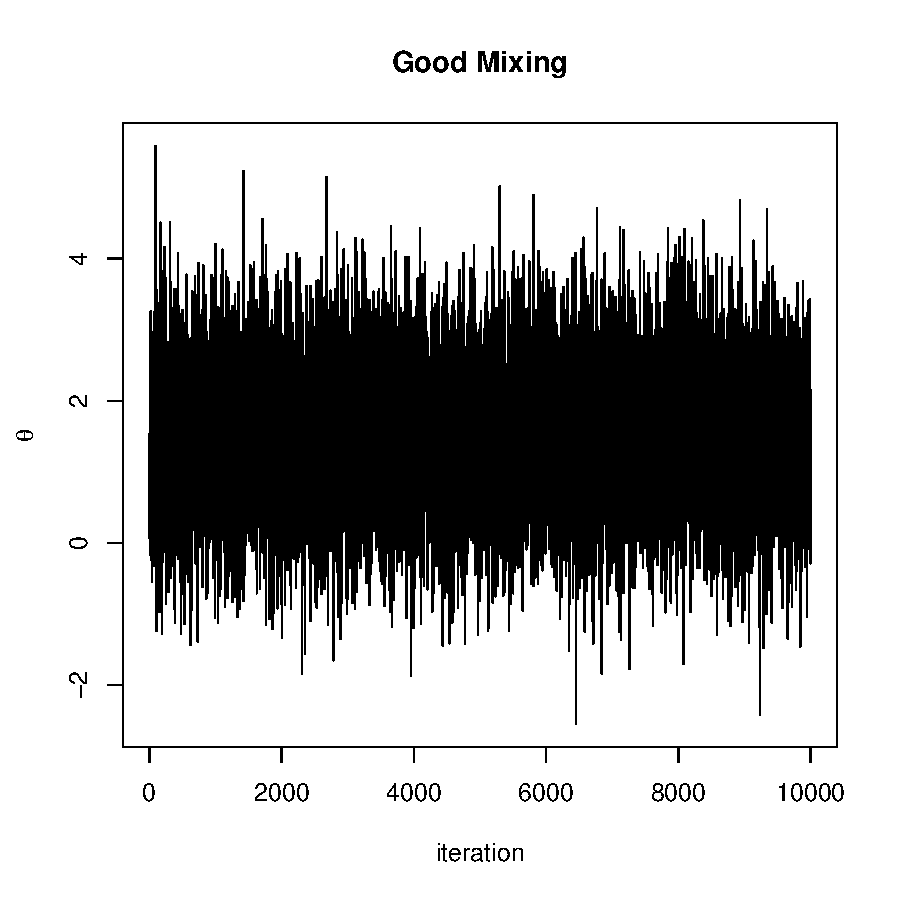
\includegraphics[width=2in, height=2in]{convergence-tracegood.pdf}}
\subfigure{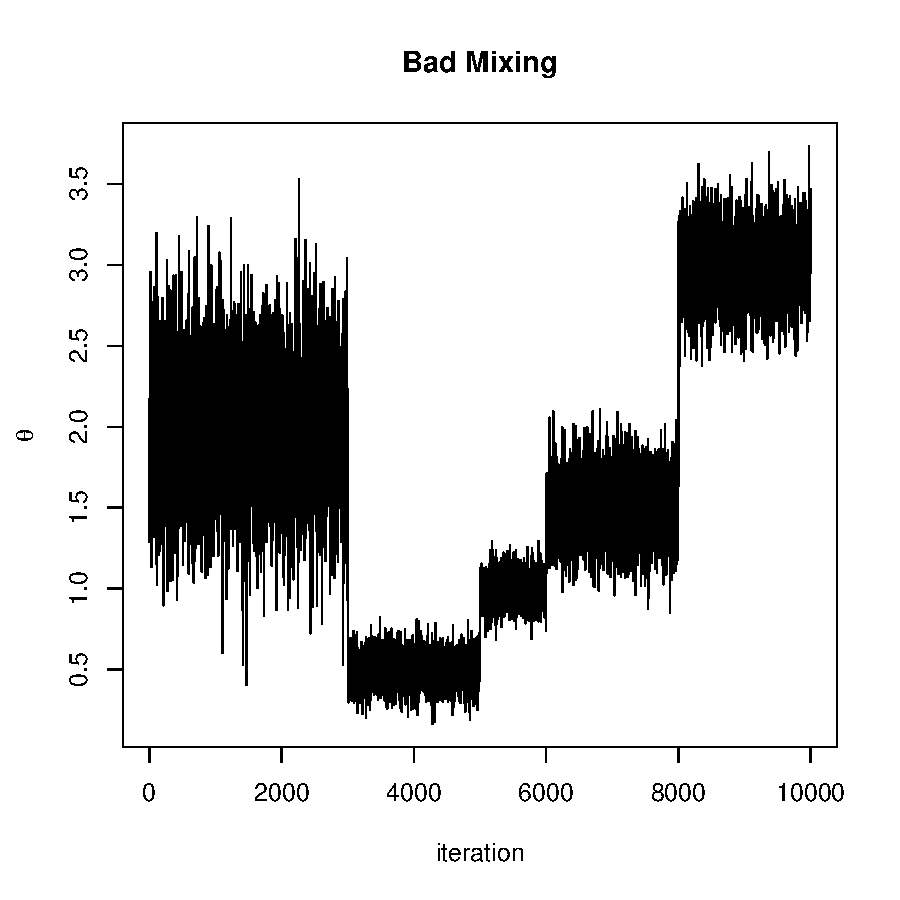
\includegraphics[width=2in, height=2in]{convergence-tracebad.pdf}}
\end{center}
\end{figure}
\end{frame}

\begin{frame}[fragile]
\frametitle{Traceplots and Density Plots}
\pause
We can do traceplots and density plots by plotting an {\tt mcmc}
object or by calling the {\tt traceplot()} and {\tt densplot()} functions.
\pause
\medskip
\tiny
\begin{Schunk}
\begin{Sinput}
> plot(mh.draws)
\end{Sinput}
\end{Schunk}
\begin{figure}[!htp]
\begin{center}
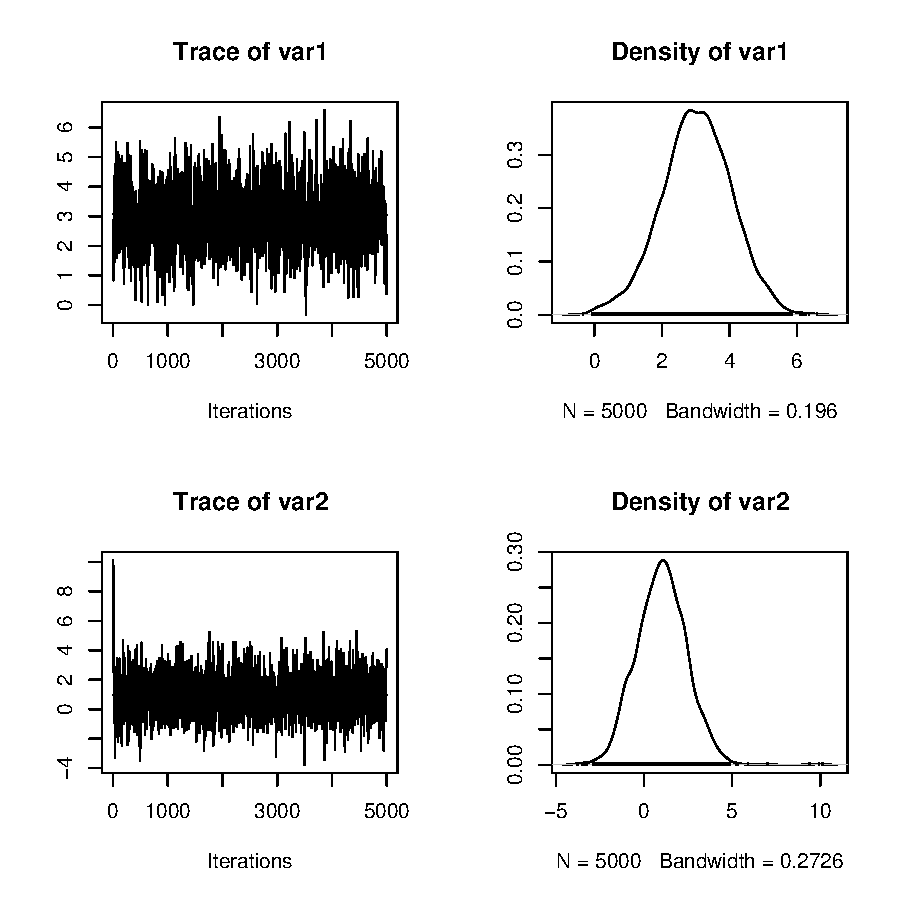
\includegraphics[width=2in, height=2in]{convergence-trace.pdf}
\end{center}
\end{figure}
\normalsize
\end{frame}


\begin{frame}
\frametitle{Running Mean Plots}
\pause
We can also use \textbf{running mean plots} to check how well our
chains are mixing. \\
\pause
\bigskip
A running mean plot is a plot of the iterations against the mean of
the draws up to each iteration.
\pause

\begin{figure}[!htp]
\begin{center}
\subfigure{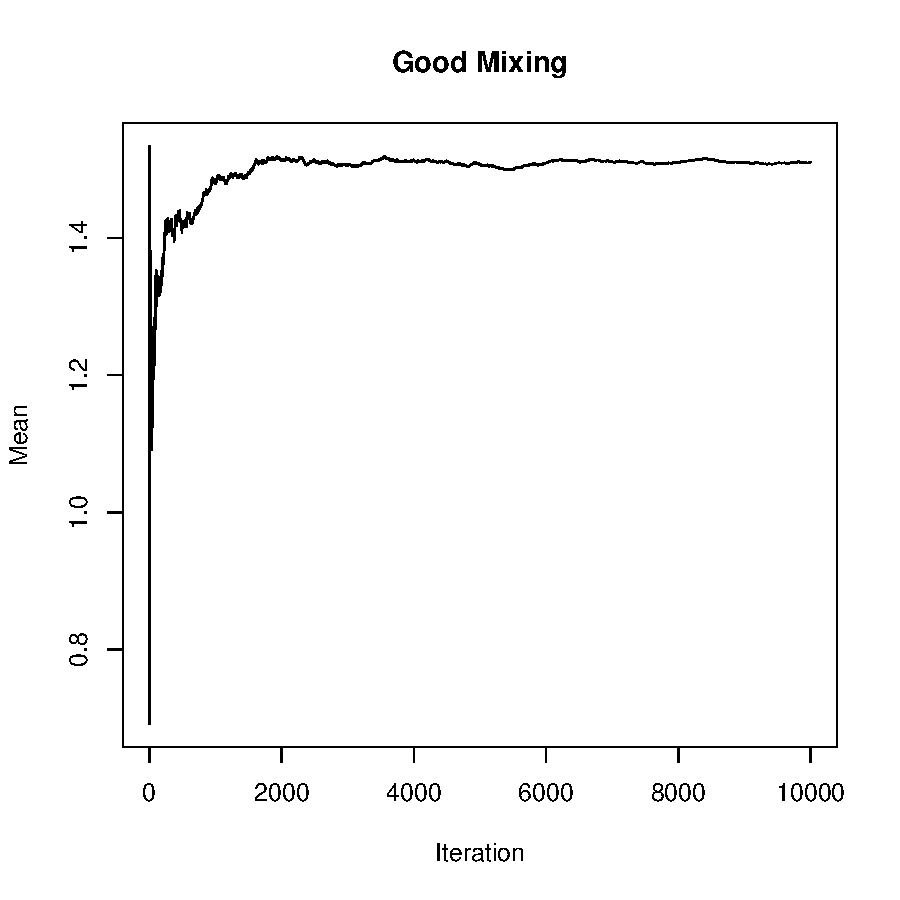
\includegraphics[width=2in, height=2in]{convergence-meangood.pdf}}
\subfigure{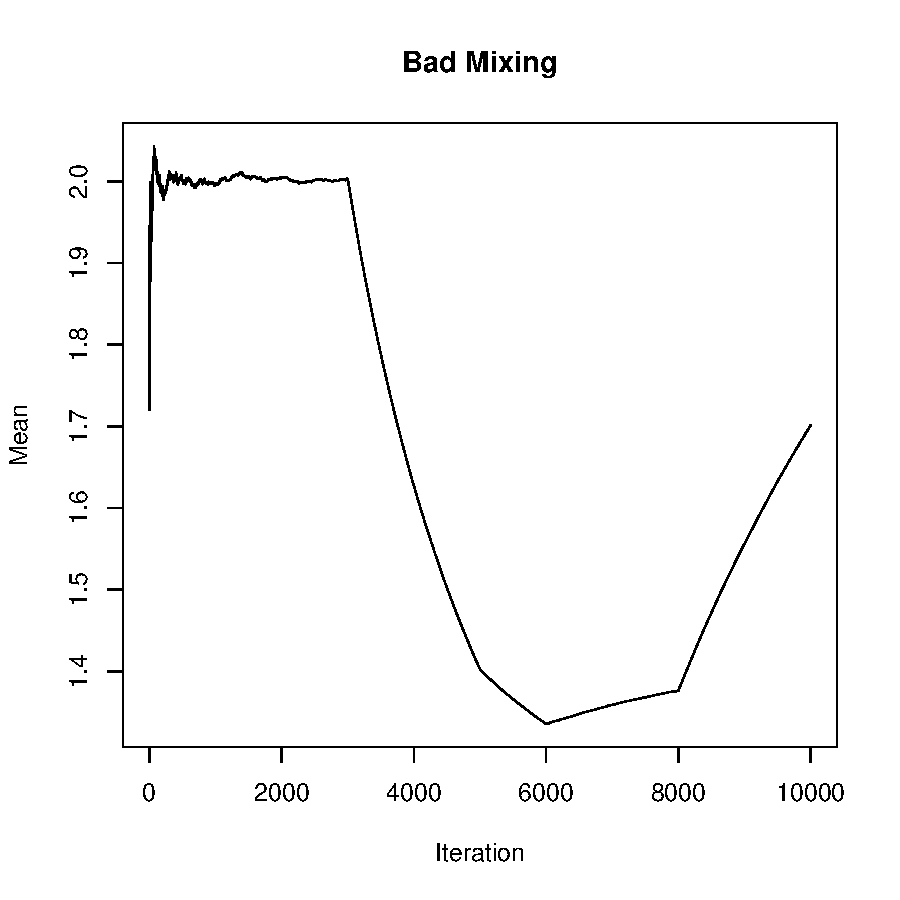
\includegraphics[width=2in, height=2in]{convergence-meanbad.pdf}}
\end{center}
\end{figure}
\end{frame}

\begin{frame}
\frametitle{Autocorrelation}
\pause
Another way to assess convergence is to assess the autocorrelations
between the draws of our Markov chain.\\
\pause
\bigskip
The lag $k$ autocorrelation $\rho_k$ is the correlation between every draw and
its $k$th lag:
\pause
\begin{eqnarray*}
\rho_k = \frac{\sum_{i=1}^{n-k} (x_i - \bar{x})(x_{i+k} -
\bar{x})}{\sum_{i=1}^n (x_i - \bar{x})^2}
\end{eqnarray*}
\pause
We would expect the $k$th lag autocorrelation to be smaller as $k$
increases \pause (our 2nd and 50th draws should be less correlated
than our 2nd and 4th draws).\\
\pause
\bigskip
If autocorrelation is still relatively high for higher values of $k$,
this indicates high degree of correlation between our draws and slow mixing.
\end{frame}

\begin{frame}

\begin{figure}[!htp]
\begin{center}
\subfigure{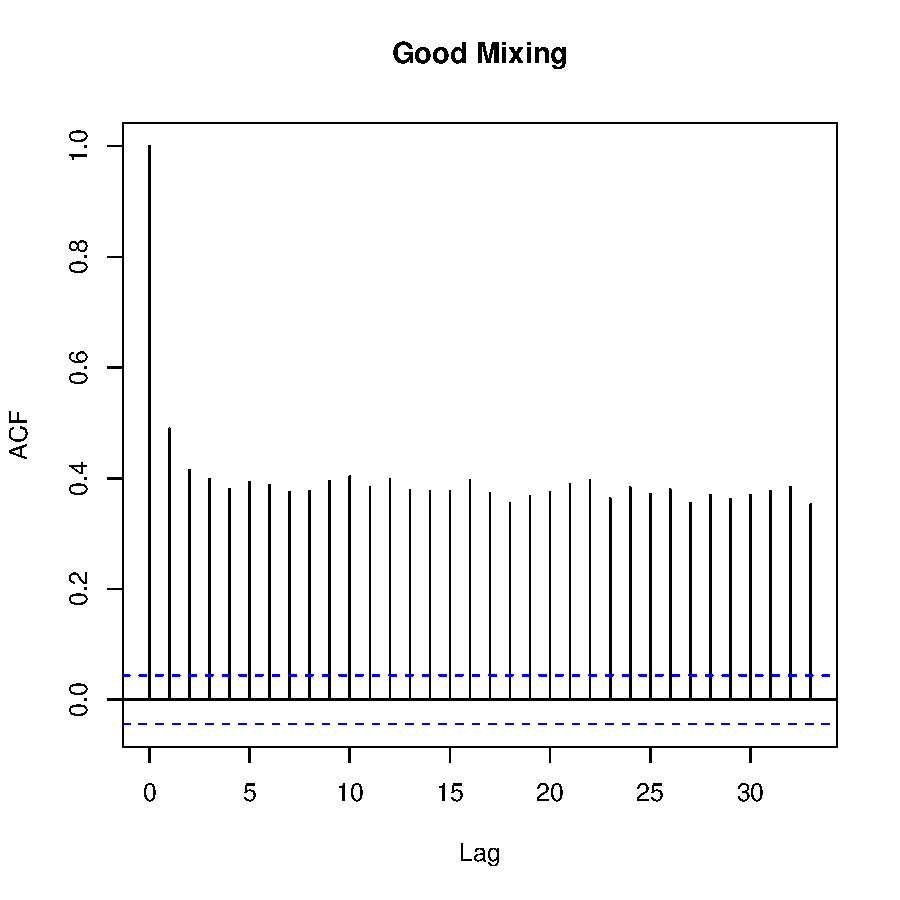
\includegraphics[width=2in, height=2in]{convergence-acfgood.pdf}}
\subfigure{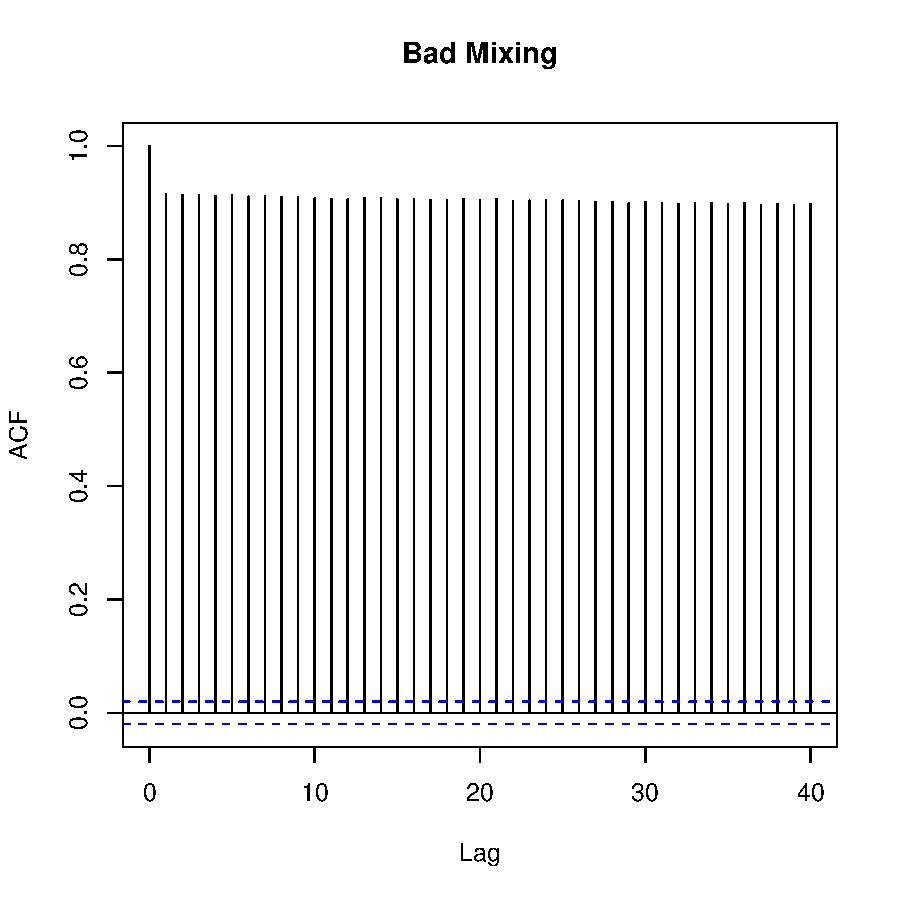
\includegraphics[width=2in, height=2in]{convergence-acfbad.pdf}}
\end{center}
\end{figure}
\end{frame}

\begin{frame}[fragile]
\frametitle{Autocorrelation Plots}
\pause
We can get autocorrelation plots using the {\tt autocorr.plot()} function.
\pause
\medskip
\tiny
\begin{Schunk}
\begin{Sinput}
> autocorr.plot(mh.draws)
\end{Sinput}
\end{Schunk}
\begin{figure}[!htp]
\begin{center}
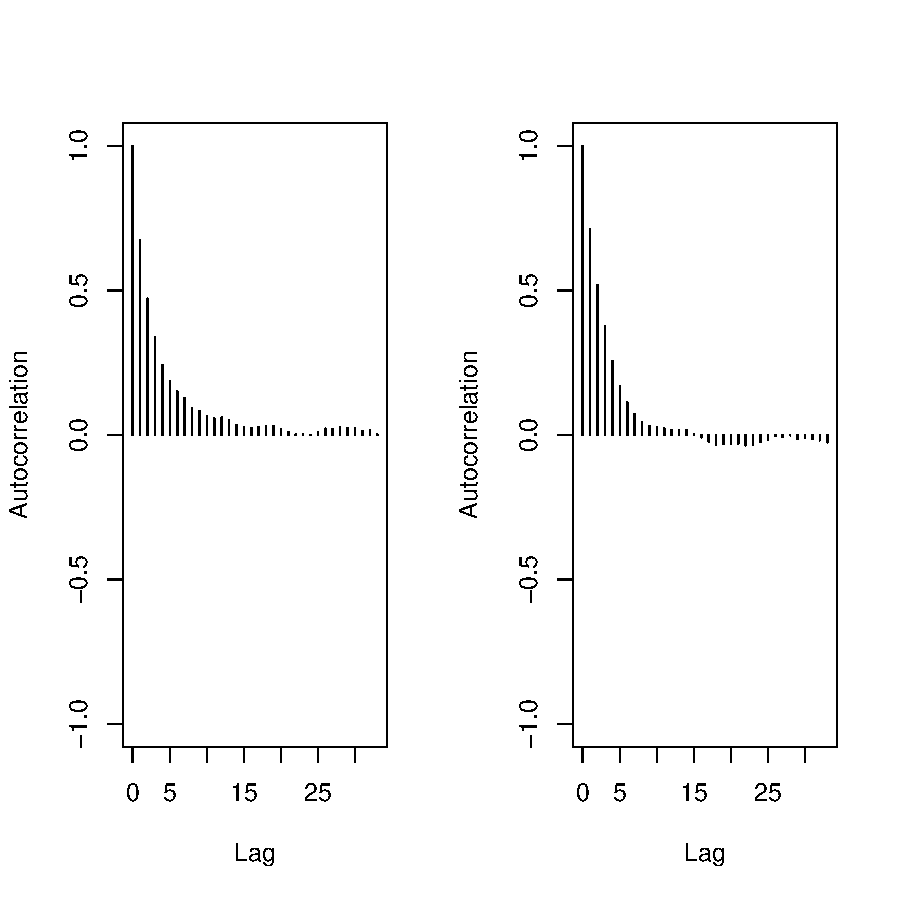
\includegraphics[width=2in, height=2in]{convergence-autocorr.pdf}
\end{center}
\end{figure}
\normalsize
\end{frame}

\begin{frame}[fragile]
\frametitle{Rejection Rate for Metropolis-Hastings Algorithm}
\pause
We can also get a rejection rate for the Metropolis-Hastings algorithm
using the {\tt rejectionRate()} function.
\pause
\medskip
\tiny
\begin{Schunk}
\begin{Sinput}
> rejectionRate(mh.draws)
\end{Sinput}
\begin{Soutput}
     var1      var2 
0.5277055 0.4094819 
\end{Soutput}
\end{Schunk}
\normalsize
\bigskip
\pause
To get the acceptance rate, we just want $1 - $ rejection rate.
\pause
\medskip
\tiny
\begin{Schunk}
\begin{Sinput}
> acceptance.rate <- 1 - rejectionRate(mh.draws)
> acceptance.rate
\end{Sinput}
\begin{Soutput}
     var1      var2 
0.4722945 0.5905181 
\end{Soutput}
\end{Schunk}
\normalsize
\end{frame}

\section{Gelman and Rubin Diagnostic}

\begin{frame}
\frametitle{Outline}
\tableofcontents[currentsection]
\end{frame}

\begin{frame}
\frametitle{Gelman and Rubin Multiple Sequence Diagnostic}
\pause
Steps (for each parameter):
\pause
\begin{enumerate}
\item Run $m \ge 2$ chains of length 2$n$ from overdispersed starting values.
\pause
\item Discard the first $n$ draws in each chain.
\pause
\item Calculate the within-chain and between-chain variance.
\pause
\item Calculate the estimated variance of the parameter as a weighted
sum of the within-chain and between-chain variance.
\pause
\item Calculate the potential scale reduction factor.  
\end{enumerate}
\end{frame}

\begin{frame}
\frametitle{Within Chain Variance}
\pause
\begin{eqnarray*}
W = \frac{1}{m} \sum_{j=1}^m s^2_j
\end{eqnarray*} 
where
\begin{eqnarray*}
s^2_j = \frac{1}{n-1} \sum_{i=1}^n (\theta_{ij} - \bar{\theta}_j)^2
\end{eqnarray*}
\pause
$s^2_j$ is just the formula for the variance of the $j$th chain.
\pause  $W$ is then just the mean of the variances of each chain.\\
\pause
\bigskip
$W$ likely underestimates the true variance of the stationary distribution
since our chains have probably not reached all the points of the
stationary distribution.
\end{frame}

\begin{frame}
\frametitle{Between Chain Variance}
\pause
\begin{eqnarray*}
B = \frac{n}{m-1} \sum_{j=1}^m (\bar{\theta}_j - \bar{\bar{\theta}})^2
\end{eqnarray*}
where
\begin{eqnarray*}
\bar{\bar{\theta}} = \frac{1}{m} \sum_{j=1}^m \bar{\theta}_j
\end{eqnarray*}
\pause
This is the variance of the chain means multiplied by $n$ because each
chain is based on $n$ draws.
\end{frame}

\begin{frame}
\frametitle{Estimated Variance}
\pause
We can then estimate the variance of the stationary distribution as a
weighted average of $W$ and $B$.
\pause
\begin{eqnarray*}
\hat{\mathrm{Var}}(\theta) = (1-\frac{1}{n}) W + \frac{1}{n} B
\end{eqnarray*}
\pause
Because of overdispersion of the starting values, this overestimates
the true variance, but is unbiased if the starting distribution equals
the stationary distribution (if starting values were not overdispersed).
\end{frame}

\begin{frame}
\frametitle{Potential Scale Reduction Factor}
\pause
The potential scale reduction factor is
\begin{eqnarray*}
\hat{R} = \sqrt{\frac{\hat{\mathrm{Var}}(\theta)}{W}}
\end{eqnarray*}
\pause
When $\hat{R}$ is high (perhaps greater than 1.1 or 1.2), then we
should run our chains out longer to improve convergence to the
stationary distribution.
\end{frame}

\begin{frame}
If we have more than one parameter, then we need to calculate the
potential scale reduction factor for each parameter.\\
\bigskip
\pause
We should run our chains out long enough so that all the potential
scale reduction factors are small enough.\\
\bigskip
\pause
We can then combine the $mn$ total draws from our chains to produce
one chain from the stationary distribution.
\end{frame}


\begin{frame}[fragile]
We can do the \textbf{Gelman and Rubin diagnostic} in R.\\
\bigskip
\pause
First, we run $M$ chains at different (should be overdispersed)
starting values ($M = 5$ here) and convert them to {\tt mcmc} objects.
\pause
\medskip
\tiny
\begin{Schunk}
\begin{Sinput}
> mh.draws1 <- mcmc(NormalMHExample(n.sim = 5000, n.burnin = 0))
> mh.draws2 <- mcmc(NormalMHExample(n.sim = 5000, n.burnin = 0))
> mh.draws3 <- mcmc(NormalMHExample(n.sim = 5000, n.burnin = 0))
> mh.draws4 <- mcmc(NormalMHExample(n.sim = 5000, n.burnin = 0))
> mh.draws5 <- mcmc(NormalMHExample(n.sim = 5000, n.burnin = 0))
\end{Sinput}
\end{Schunk}
\normalsize
\bigskip
\pause
We then put the $M$ chains together into an {\tt mcmc.list}.
\pause
\medskip
\tiny
\begin{Schunk}
\begin{Sinput}
> mh.list <- mcmc.list(list(mh.draws1, mh.draws2, mh.draws3, mh.draws4, 
+     mh.draws5))
\end{Sinput}
\end{Schunk}
\normalsize
\end{frame}

\begin{frame}[fragile]
We then run the diagnostic with the {\tt gelman.diag()} function.
\pause
\medskip
\tiny
\begin{Schunk}
\begin{Sinput}
> gelman.diag(mh.list)
\end{Sinput}
\begin{Soutput}
Potential scale reduction factors:

     Point est. 97.5% quantile
[1,]       1.00           1.00
[2,]       1.00           1.00

Multivariate psrf

1.00
\end{Soutput}
\end{Schunk}
\normalsize
\bigskip
\pause
The results give us the median potential scale reduction factor and
its $97.5\%$ quantile (the psrf is estimated with uncertainty because
our chain lengths are finite).  \\
\bigskip
\pause
We also get a multivariate potential scale reduction factor that was
proposed by Gelman and Brooks.\footnote{\tiny Brooks, Stephen P. and
Andrew Gelman. 1997. ``General methods for monitoring convergence of iterative simulations.'' \textit{Journal of Computational and Graphical Statistics} 7: 434-455. }
\end{frame}

\begin{frame}[fragile]
\normalsize
We can see how the potential scale reduction factor changes through
the iterations using the {\tt gelman.plot()} function.
\pause
\medskip
\tiny
\begin{Schunk}
\begin{Sinput}
> gelman.plot(mh.list)
\end{Sinput}
\end{Schunk}
\begin{figure}[!htp]
\begin{center}
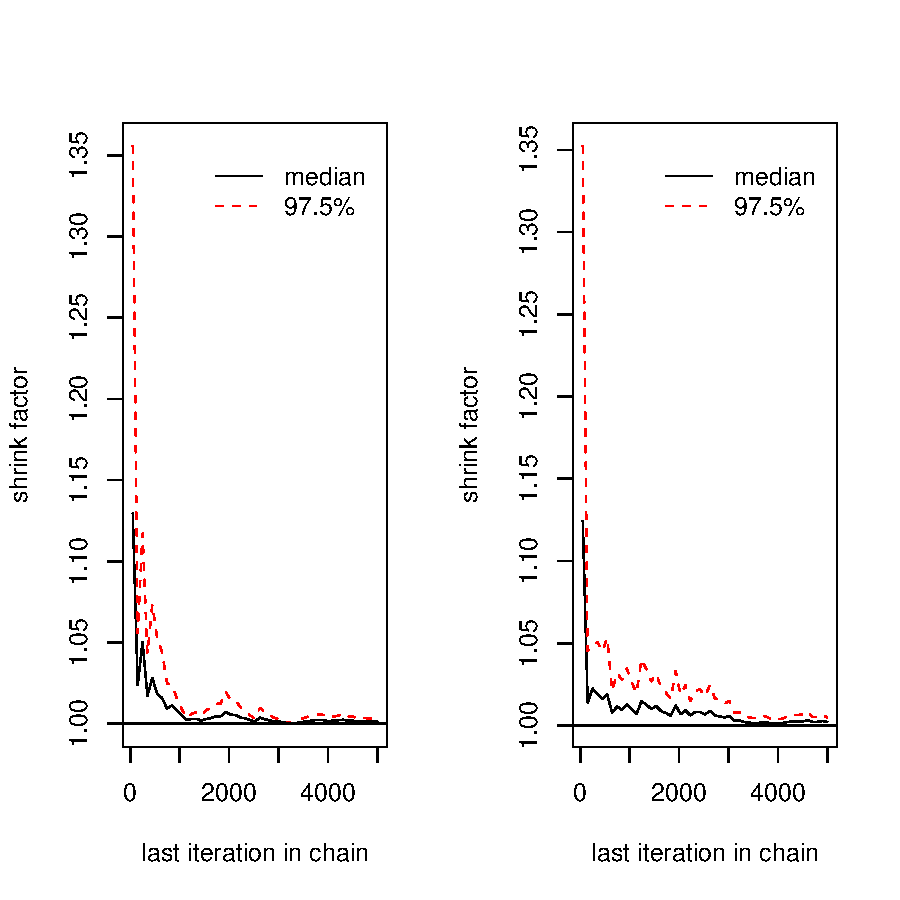
\includegraphics[width=2in, height=2in]{convergence-gelman.pdf}
\end{center}
\end{figure}
\normalsize
\end{frame}


\section{Geweke Diagnostic}

\begin{frame}
\frametitle{Outline}
\tableofcontents[currentsection]
\end{frame}

\begin{frame}[fragile]
\frametitle{Geweke Diagnostic}
\pause
The \textbf{Geweke diagnostic} takes two nonoverlapping parts (usually
the first 0.1 and last 0.5 proportions) of the
Markov chain and compares the means of both parts, using a
difference of means test to see if the two parts of the chain are from
the same distribution (null hypothesis). \\
\pause
\bigskip
The test statistic is a standard Z-score with the standard errors
adjusted for autocorrelation. \\
\pause
\bigskip
\tiny
\begin{Schunk}
\begin{Sinput}
> geweke.diag(mh.draws)
\end{Sinput}
\begin{Soutput}
Fraction in 1st window = 0.1
Fraction in 2nd window = 0.5 

  var1   var2 
0.6149 0.1035 
\end{Soutput}
\end{Schunk}
\normalsize 
\end{frame}

\section{Raftery and Lewis Diagnostic}

\begin{frame}
\frametitle{Outline}
\tableofcontents[currentsection]
\end{frame}

\begin{frame}
\frametitle{Raftery and Lewis Diagnostic}
\pause
Suppose we want to measure some posterior quantile of interest $q$.\\
\bigskip
\pause 
If we define some acceptable tolerance $r$ for $q$ and a
probability $s$ of being within that tolerance, the \textbf{Raftery
and Lewis
diagnostic} will calculate the number of iterations $N$ and the number of
burn-ins $M$ necessary to satisfy the specified conditions.\\
\bigskip
\pause
The diagnostic was designed to test the number of iterations and burn-in needed by first running and testing shorter pilot chain. \\
\bigskip
\pause
In practice, we can also just test our normal chain to see if it
satisfies the results that the diagnostic suggests.
\end{frame}

\begin{frame}
\frametitle{Inputs:}
\pause
\begin{enumerate}
\item Select a posterior quantile of interest $q$ (for example, the
0.025 quantile).
\pause
\item Select an acceptable tolerance $r$ for this quantile \pause (for
example, if $r = 0.005$, then that means we want to measure the
$0.025$ quantile with an accuracy of $\pm 0.005$).
\pause
\item Select a probability $s$, which is the desired probability of
being within (q-r, q+r).
\pause
\item Run a ``pilot'' sampler to generate a Markov chain of minimum
length given by rounding up
\begin{eqnarray*}
n_{\mathrm{min}} = \left[ \Phi^{-1} \left( \frac{s+1}{2} \right)
\frac{\sqrt{q(1-q)}}{r} \right] ^2
\end{eqnarray*}
where $\Phi^{-1} (\cdot)$ is the inverse of the normal CDF.
\end{enumerate}
\end{frame}

\begin{frame}[fragile]
\frametitle{Results:}
\pause
\tiny
\begin{Schunk}
\begin{Sinput}
> raftery.diag(mh.draws, q = 0.025, r = 0.005, s = 0.95)
\end{Sinput}
\begin{Soutput}
Quantile (q) = 0.025
Accuracy (r) = +/- 0.005
Probability (s) = 0.95 
                                       
 Burn-in  Total Lower bound  Dependence
 (M)      (N)   (Nmin)       factor (I)
 18       20149 3746         5.38      
 13       14570 3746         3.89      
\end{Soutput}
\end{Schunk}
\normalsize
\pause
\begin{itemize}
\item $M$: number of burn-ins necessary
\pause
\item $N$: number of iterations necessary in the Markov chain
\pause
\item $N_{\mathrm{min}}$: minimum number of iterations for
the ``pilot'' sampler
\pause
\item I: dependence factor, interpreted as the proportional increase
in the number of iterations attributable to serial dependence.  \\
\pause
\bigskip
High dependence factors ($> 5$) are worrisome and may be due to
influential starting values, high correlations between coefficients,
or poor mixing.
\end{itemize}
\end{frame}

\begin{frame}
The Raftery-Lewis diagnostic will differ depending on which quantile
$q$ you choose. \\
\pause
\bigskip
Estimates tend to be conservative in that it will suggest more
iterations than necessary. \\
\pause
\bigskip
It only tests marginal convergence on each parameter. \\
\pause
\bigskip
Nevertheless, it often works well with simple models.
\end{frame}

\section{Heidelberg and Welch Diagnostic}

\begin{frame}
\frametitle{Outline}
\tableofcontents[currentsection]
\end{frame}

\begin{frame}
\frametitle{Heidelberg and Welch Diagnostic}
\pause
The \textbf{Heidelberg and Welch diagnostic} calculates a test statistic
(based on the Cramer-von Mises test statistic) to accept or reject the
null hypothesis that the Markov chain is from a stationary distribution.\\
\pause
\bigskip
The diagnostic consists of two parts.
\end{frame}

\begin{frame}
\frametitle{First Part:}
\pause
\begin{enumerate}
\item Generate a chain of $N$ iterations and define an $\alpha$ level.
\pause
\item Calculate the test statistic on the whole chain.  Accept or
reject null hypothesis that the chain is from a stationary distribution.
\pause
\item If null hypothesis is rejected, discard the first $10\%$ of the
chain.  Calculate the test statistic and accept or reject null.
\pause
\item If null hypothesis is rejected, discard the next $10\%$ and
calculate the test statistic.  
\pause
\item Repeat until null hypothesis is accepted or $50\%$ of the chain
is discarded.  If test still rejects null hypothesis, then the chain
fails the test and needs to be run longer.
\end{enumerate}
\end{frame}

\begin{frame}[fragile]
\frametitle{Second Part:}
\pause
If the chain passes the first part of the diagnostic, then it takes
the part of the chain not discarded from the first part to test the second part.\\
\bigskip
\pause
The halfwidth test calculates half the width of the $(1-\alpha)\%$
credible interval around the mean.  \\
\bigskip
\pause
If the ratio of the halfwidth and the mean is lower than some
$\epsilon$, then the chain passes the test.  Otherwise, the chain must
be run out longer.
\pause
\bigskip
\tiny
\begin{Schunk}
\begin{Sinput}
> heidel.diag(mh.draws)
\end{Sinput}
\begin{Soutput}
     Stationarity start     p-value
     test         iteration        
var1 passed       1         0.834  
var2 passed       1         0.693  
                             
     Halfwidth Mean Halfwidth
     test                    
var1 passed    3.03 0.0756   
var2 passed    1.00 0.0805   
\end{Soutput}
\end{Schunk}
\normalsize 
\end{frame}


\end{document}













